\documentclass{report}

\input{preamble}
\input{macros}
\input{letterfonts}

\usepackage{tikz}
\usepackage{tikz-3dplot}
\usepackage{amsmath}
\usepackage{amssymb}
\usepackage{pgfplots}
\usepgfplotslibrary{polar}
\pgfplotsset{compat=newest}
\usepackage{smartdiagram}
\usepackage{xcolor}
\usepackage{forest}
\usepgfplotslibrary{colormaps}
\usepgfplotslibrary{groupplots}

\usesmartdiagramlibrary{additions}

\title{\Huge{Temporary Doc}\\Calc 3}
\author{\huge{Giacomo Cappelletto}}
\date{23/10/24}

\begin{document}


\maketitle
\pagebreak
\pdfbookmark[section]{\contentsname}{toc}
\tableofcontents
\pagebreak

\chapter{Vector Valued Functions $f:\mathbb{R} \rightarrow \mathbb{R}^n$}

\section{Arc Length in Polar Coordinates}

The position vector in polar coordinates is given by:
\[
	\vec{r}(t) = \langle f(\theta) \cos\theta, f(\theta) \sin\theta \rangle
\]

The magnitude of the derivative of the position vector is:
\[
	|\vec{r}'(t)| = \sqrt{ \left( f'(\theta) \cos\theta - f(\theta) \sin\theta \right)^2
		+ \left( f'(\theta) \sin\theta + f(\theta) \cos\theta \right)^2 }
\]

Simplifying, this becomes:
\[
	|\vec{r}'(t)| = \sqrt{ \left( f'(\theta) \right)^2 + \left( f(\theta) \right)^2 }
\]

The arc length \(S_r\) is then calculated as:
\[
	S_r = \int_{\theta_1}^{\theta_2} \sqrt{\left(f'(\theta)\right)^2 + \left(f(\theta)\right)^2} \, d\theta
\]


\ex{Circle of Radius \(a\)}{

	\textbf{Example:} Let \(r(\theta) = a\), where:
	\[
		r'(\theta) = 0, \quad r(\theta) = a
	\]
	The arc length is:
	\[
		S = \int_0^{2\pi} \sqrt{a^2} \, d\theta = a \int_0^{2\pi} 1 \, d\theta = 2\pi a
	\]
}


\section{Multivariate Case}

The double integral over a region \(R\):
\[
	\iint_R f(x, y) \, dA
\]
If converted to polar coordinates:
\[
	\iint_R f(x, y) \, dA = \iint_R f(r\cos\theta, r\sin\theta) \, r \, dr \, d\theta
\]

\ex{Volume under \(z = 9 - x^2 - y^2\):}{

	\[
		R = \{(x, y): x^2 + y^2 \leq 9\}
	\]
	In polar coordinates:
	\[
		R = \{(r, \theta): 0 \leq \theta \leq 2\pi, 0 \leq r \leq 3\}
	\]

	The function in polar coordinates:
	\[
		f(r, \theta) = 9 - r^2
	\]

	The volume is then:
	\[
		\int_R f(r, \theta) \, dA = \int_0^{2\pi} \int_0^3 r(9 - r^2) \, dr \, d\theta
	\]

	\begin{center}
		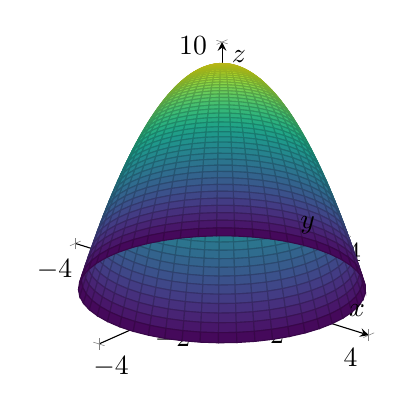
\begin{tikzpicture}
			\begin{axis}[
					view={40}{30},
					axis lines=middle,
					xlabel={$x$},
					ylabel={$y$},
					zlabel={$z$},
					zmin=0, zmax=10, xmin=-4, xmax=4, ymin=-4, ymax=4,
					samples=50
				]
				\addplot3[
					domain=0:360,
					y domain=0:3,
					surf,
					colormap/viridis
				]
				({y*cos(x)},{y*sin(x)},{9-y^2});
			\end{axis}
		\end{tikzpicture}
	\end{center}

	\textbf{Simplified Polar Volume Calculation:}
	\[
		\int_R f(r, \theta) \, dA = \int_0^{2\pi} \int_0^3 r(9 - r^2) \, dr \, d\theta
	\]

}

\section{General Procedure for Polar Integration}

Given a region \( R = \{(r, \theta): \theta_1 \leq \theta \leq \theta_2, \, q(\theta) \leq r \leq h(\theta)\} \), the volume is calculated as:
\[
	V = \iint_R f(r, \theta) \, dA = \int_{\theta_1}^{\theta_2} \int_{q(\theta)}^{h(\theta)} r f(r, \theta) \, dr \, d\theta
\]
where the area element is \( \Delta A = r \, \Delta r \, \Delta \theta \).

\ex{Example: Region Outside \(r = \frac{1}{2}\) and Inside \(r = 1 + \cos\theta\)}{

\textbf{The bounds are:}
\[
	\frac{1}{2} \leq r \leq 1 + \cos\theta
\]
\[
	-\frac{2\pi}{3} \leq \theta \leq \frac{2\pi}{3}
\]

\textbf{Cosine conditions are determined by:}
\[
	\cos\theta = -\frac{1}{2}, \quad \theta = -\frac{2\pi}{3}, \, \frac{2\pi}{3}
\]

The integral for the volume is:
\[
	\iint_R q(r, \theta) \, dA = \int_{-\frac{2\pi}{3}}^{\frac{2\pi}{3}} \int_{\frac{1}{2}}^{1+\cos\theta} r \, q(r, \theta) \, dr \, d\theta
\]


\begin{center}
    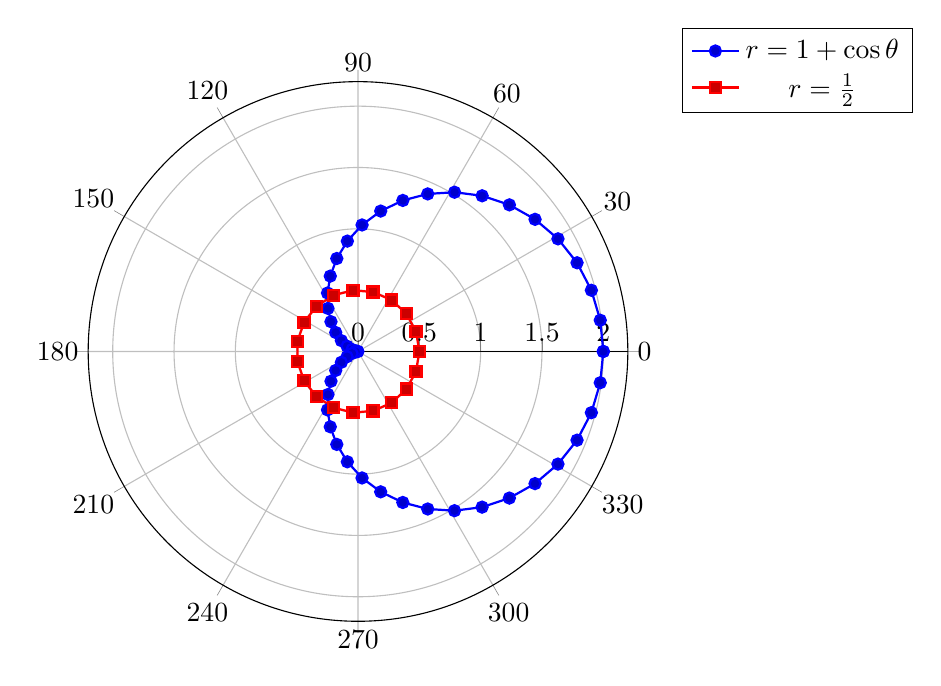
\begin{tikzpicture}
        \begin{polaraxis}[
                legend style={at={(1.1,1.1)}, anchor=north west}
            ]
            % Plot the curve r = 1 + cos(theta)
            \addplot+[domain=0:360, samples=50, thick, blue] (x, {1 + cos(x)});
            \addlegendentry{$r = 1 + \cos\theta$}

            \addplot+[domain=0:360, samples=20, thick, red] ({x},{0.5});
            \addlegendentry{$r = \frac{1}{2}$}

        \end{polaraxis}
    \end{tikzpicture}
\end{center}
}

\end{document}